\documentclass[12pt,a4paper,english,twoside]{book}
\usepackage[german,english]{babel}
\usepackage[T1]{fontenc} 
\usepackage[utf8]{inputenc}
\usepackage{amsfonts}
\usepackage{amsmath}
\usepackage{amsthm}
\usepackage{latexsym}
\usepackage{amssymb}
\usepackage{epsfig}
\usepackage{moreverb}
\usepackage{rotating}
\usepackage{enumerate}
\usepackage{graphics, graphicx, wrapfig}
\usepackage{fancybox}
\usepackage{picinpar,varioref,floatflt}
\usepackage{ae}
\usepackage{longtable}
\usepackage{textcomp}
\usepackage{float}
\usepackage{url}
\usepackage{unizhdt}
\usepackage{framed}
\usepackage{caption}
\usepackage{algorithm}
\usepackage[noend]{algpseudocode}


\usepackage{lipsum}
\usepackage[svgnames]{xcolor}
\usepackage[tikz]{bclogo}



%%%%%%%%%%%%%%%%%%%%%%%%%%%%%%%%%%%%%%%%%%%%%%%%%%

% Define the language of the diploma thesis
\selectlanguage{english}

\pagestyle{headings}

\begin{document}

%%%%%%%%%%%%%%%%%%%%%%%%%%%%%%%%%%%%%%%%%%%%%%%%%%

% Define the author printed on the cover page
\author{Jan von der Assen}
% Define the city and country of the author
\authorcity{Zurich, Switzerland}
% Define the student ID (Matrikelnummer)
\studentid{14-719-132}
% Define the title with optional subtitle
\title{A Progressive Web App (PWA)-based Mobile Wallet for Bazo}
% Define the supervisors
\supervisors{Thomas Bocek, Bruno Rodrigues, Hamza Bedrija}
% Define the submission date
\submissiondate{January 31, 2018}

%%%%%%%%%%%%%%%%%%%%%%%%%%%%%%%%%%%%%%%%%%%%%%%%%%

% Make the title page
\maketitle

% Make the imprint on the back of the cover page
\makeimprint

\pagenumbering{roman}

% Include the files of the diploma thesis
%\cleardoublepage
\chapter*{Abstract}
\addcontentsline{toc}{chapter}{Abstract}

\selectlanguage{english}
Ein Finanzdienstleister aus Zürich unterhält ein Bonusprogramm um die Verwendung von Kredit- und Debitkarten zu belohnen. Der traditionelle Prozess wie Bonuspunkte gegen Produkte getauscht werden können, bedeutete, dass Verträge zu Partnerfirmen unterhalten werden müssen. Dieser Prozess führte dazu, dass das Programm bei Kunden kaum bekannt wurde. Aus diesem Grund wurde an der Universität Zürich die Bazo Krypto-Währung entwickelt, welche nur eingeladenen Teilnehmern offen steht. Um den Finanzdienstleister die Technologie evaluieren zu lassen, wurden weitere Entwicklungsaufwände betrieben um andere übliche Applikationen für Kryptowährungen bereitzustellen. Der Fokus dieser Arbeit liegt auf der Planung, Entwicklung und Evaluation einer Zahlungs-Applikation für die Bazo Währung. Neben dieser Entwicklung befasst sich diese Arbeit auch mit der Erfassung des aktuellen Stands von Web APIs, die normalerweise nur auf nativen Applikationen zur Verfügung stehen. Weiter wurde untersucht wie native APIs einer Web Applikation zur Verfügung gestellt werden können. Konkret wurde dazu ein Proof-of-Concept erstellt, womit native Funktionen einer Web Applikation bereit gestellt werden. Weiter wurden Schnittstellen zu existierenden Systemen, wie dem Bonusprogramm und der Kryptowährung, geplant und entwickelt. Ausserdem wurde im Rahmen der Arbeit evaluiert wie die existierende Client Applikation auf das mobile Betriebssystem Android portiert werden kann.
\selectlanguage{english}

A financial service provider in Zurich maintains a bonus program to incentivize credit and debit card usage. The process of exchanging bonus points against goods implied efforts to maintain contracts with partners and led to low usage of the program by customers. This led to the development of the Bazo cryptocurrency at the University of Zurich, which is an invite-only, blockchain-based currency. In order to let the financial service provider evaluate the technology, further development efforts were taken to enrich the ecosystem of the currency. The scope of this thesis is the design, development and evaluation of a web-based payment application for the Bazo cryptocurrency. Besides the development of the application, this thesis explores related topics, such as a comparison of Web APIs with native APIs by developing a Proof of Concept for the Android operating system. Further, the development efforts for the required interfaces to the currency and to the companys existing infrastructure are described. Finally, a mobile port of the existing client application for the Bazo currency targeted to the Android operating system was created and evaluated.

%%paper?%%
%\cleardoublepage
\chapter*{Acknowledgments}
\addcontentsline{toc}{chapter}{Acknowledgments}

I would like to express my gratitude to my supervisor, Dr. Thomas Bocek, for sharing his passion and experience within the project. He has always provided an interesting view on various topics and thus made this thesis an exciting opportunity.

Further, I would like to thank the other members of the project for their competent work and collaboration.

Lastly, I would like to thank Prof Dr. Burkhard Stiller, head of the Communication Systems Group, for making it possible to write my thesis within the scope of this project.


\tableofcontents

\cleardoublepage
\pagenumbering{arabic}
\chapter{Introduction}
%% Importance etc of Blockchain based currencies

A financial service provider based in Zurich developed a bonus program that incentivizes customers to use its credit and debit cards. With every completed purchase, customers collect virtual points. Several industry partners are participants of this bonus program. The virtual points collected can be exchanged for gift cards from partners registered via the Web site or an app. The way that these services can be used in the traditional system puts the company into a central role, thus requiring administrative efforts to enable both customers and partners to exchange virtual points. In order to decentralize the financial service provider's position, a blockchain based currency, Bazo (Esperanto: base; foundation), was developed at the University of Zurich. The intention of the currency is to map virtual points to coins in the crypto currency \cite{lisg}.
The focus of this thesis lies on the implementation and evaluation of a Mobile Wallet for said currency. Requirements and implementation details are gathered during the project in an explorative way in partnership with the company.
\section{Motivation}
Traditional payment systems require a centralized institution in order to maintain a currency and support operations such as issueing, transferring and determining state of currency units. Requiring the issuer for each operation that can be performed on the virtual currency further prohibits the direct trading of virtual points between users.
In the case of the partner company this resulted in a limited awareness and usage of the incentivization program by customers as well as partners.
With the new cryptocurrency developed at the University of Zurich which is tailored to the requirements of a financial service provider, it is possible to still maintain control over the currency since the company remains in an issuer position. In order to let end users such as customers and partners interact with the currency as well as making the program more transparent, further development efforts are taken. With the completion of said efforts, a first complete prototype of a currency ecosystem should be available for evaluation. That way the financial service provider can evaluate the new solution with real costumers and gain insight on how blockchain technologies can be used to improve payment processes. These development efforts involve the development of a client application to let users trade Bazo coins as well as to improve the payment process, since mobile system's capabilites for sharing transaction data can be used.

\section{Description of Work}
This thesis covers the design, implementation, and evaluation of a mobile wallet for the Bazo cryptocurrency. In order to run the client as trustless as possible, a light client implementation needs to be integrated to the Bazo wallet. This involves the integration and development of interfaces with other application in the cryptocurrency to enable operations on the blockchain.
The development should leverage existing resources from similar projects where a Mobile Wallet was implemented.
It is required to find a way to transmit payment information with native elements such as NFC and Bluetooth. However, a fallback solution needs to be implemented to allow a broad range of users to participate in the program.
In order to support the complete use case for customers and partners, it is required to integrate existing web services from the service provider. This is intended to support the complete payment process for proximity-based transfers.
The application needs to be tested in a pilot project where the Bazo cryptocurrency is used for payments in a sandboxed environment.

\section{Outline}
The main section of the report is structered as follows:
In chapter 2 an introduction to leveraged and related technologies as well as the traditional and envisioned transaction process is given. The chapter further contains a documentation of elicited and derived requirements and an analysis thereof. Further, related work as well as other activities in the project are introduced. Chapter 3 focuses on the design of a Mobile Wallet that satisfies the aforementioned requirements. The concrete implementation of the design is explained in chapter 4. In chapter 5 the prototype and the findings from developing the Wallet are evaluated and the results compared.
Chapter 6 summarizes and concludes the report.
\chapter{Background and Related Work}
This chapter aims to provide the reader with the necessary knowledge about related technologies, development activities and the initial situation of the context of this thesis. 
\section{Background}
This chapter familiarizes the reader with core concepts and technologies, which were leveraged for the development of the Bazo Wallet. An insight into the traditional and envisioned system of the financial service provider is also given, so that the reader is introduced to the company's domain.

\subsection{Web based Wallets}
A web based Wallet is a web application that allows for certain operations on the Blockchain of a currency. There are two common ways of implementing operations in the context of the web.
The first one is known as a \textit{Web Client} and allows users to operate on the Blockchain using a web application. The key difference of this approach is that assets, such as private keys, are stored on the server of the application. Since the user has to share these assets with a third party, he will lose control over his funds and is dependent on the provider. This means that funds can be stolen from users, which has happened multiple times in Web clients for the Bitcoin network \cite{masteringbitcoin}.
The second approach is known as a \textit{Signing-Only Client}. These applications do not maintain the blockchain or parts of it, as it is common with Full- or Headers-only clients. This allows to implement operations with minimal resources such as storage or network usage. Cryptographic operations are performed with the tools available in web applications and implemented in JavaScript.
A drawback of such signing-only applications is that there still needs to be a certain amount of trust with the server, that actually maintains parts of the blockchain and exposes an interface for the web applications \cite{bitcoinclients}.
Both client variants are compared in Table \ref{table:clientstable}.
%endA%
\subsection{Progressive Web Applications}\label{pwacharacteristics}
A Progressive Web Application (PWA), is a web application that has various characteristics that are usually found within native applications.
They leverage the accessibility from the web but have various enhancements to give them a user experience that is closer to native mobile applications.

A PWA can be characterized as \cite{pwas}:

%how to cite theorems?%
\theoremstyle{definition}
\newtheorem*{theorem-progressive}{Progressive}
\newtheorem*{theorem}{Connectivity Independent}
\newtheorem*{theorem-install}{Installable}
\newtheorem*{theorem-secure}{Secure}

\begin{theorem-progressive}
A PWA should be progressively enhanced, based on what the user agent supports.
\end{theorem-progressive}

\begin{theorem}
A Progressive Web Application should always present something to the user. By employing an app-shell architecture, the application can be separated from its content. The application shell as well as cached content should always be shown.
\end{theorem}
\begin{theorem-install}
A Progressive Web Application should be installable to the users home screen and accessible from there.

\end{theorem-install}
\begin{theorem-secure}
Since web application have access to powerful APIs in the browsers context, PWA's are supposed to be served from secure contexts. This can be achieved by using protocols such as \textit{https} or \textit{wss} \cite{securitychrome}.

\end{theorem-secure}
\subsection{Traditional payment process}
In the traditional process, customers were incentivized to use debit and credit cards issued by the company by rewarding the customer with points of a virtual currency based on the transaction volumes.
Through contracts that are established between the company and partner companies, the company can trade the customers virtual points against gift cards from partner companies.
Based on the terms established in the contract, the partner companies are disbursed for the value of the gift cards, which customers can redeem at the partner company.
Similar to the process of exchanging virtual points for goods, the company also has to act as a middleman when users want to exchange their points amongst each other. Both these cases pose a significant administrative effort for the company. Further disadvantages are the limited transparency of the program to users and that the virtual points have a relative short life cycle \cite{lisg}.

\subsection{Envisioned payment process}\label{envisionedpaymentprocess}
The envisioned system is supposed to overcome the stated disadvantages, by mapping the virtual points to a currency that can be used directly to make transactions between users or between user and the partner company.
The company rewarding with the virtual points should still remain in a central position for the currency and control aspects such as issueing new units and accounts.
The Wallet that is developed for making transactions with the currency is required to support user to user transactions as well as transactions between a user and the merchant. This implies that there is a way that both merchants and users can request money by exchanging payment information in a device-to-device manner. Since merchants may have more advanced payment systems, a possibility to integrate third party interfaces into the payment process is required. The detailed requirements needed to be explored with the company and are further described in Chapter \ref{functionalreq}.


\section{Related Work}
The development of a Wallet for the cryptocurrency, which is the focus of this thesis, was started when various parts of the ecosystem of the Bazo currency had already been implemented. This section introduces other applications and their role or influence on the Bazo ecosystem.
\subsection{Bazo}
Bazo is a cryptocurrency developed at the University of Zurich. The currency was tailored to the use case of the financial service provider which acts as a central institution that is able to create new coins and accounts. This makes the currency private, since an invitation needs to be used to participate. This differs from various popular cryptocurrencies such as Bitcoin and Ethereum which are both open to the public. Similar to the approach taken in Ethereum, Bazo implements an account-based data model. Consensus in the Bazo network is achieved through a Proof of Work algorithm, although there are drawbacks from employing this strategy \cite{lisg}. More information about the current state of research concerning the consensus protocol is given in the \textit{Proof of Stake} thesis \cite{proofofstake}.
The outcome of the first development efforts for Bazo consisted of two applications. The first one, \textit{Bazo Miner}, can be classified as a Mining client. The second application is a Full client \cite{bitcoinclients}. Table \ref{table:clientstable} compares the two applications.
\subsection{Bazo Client Implementations}
As part of the initial development efforts for Bazo, a full client application was created. With this application it is possible to issue transactions. However, in order to participate in the Bazo network, peers have to obtain a complete copy of the Blockchain. In order to increase applicability for various use cases and to comply with resource constraints a light client implementation is developed at the University of Zurich. With this fork implementation of the full client, peers are not required to obtain all information from the blockchain. Validation of the requested information is still ensured by employing new techniques. This opens new use cases; for example, a Bazo client can be run on a device with limited resources such as a mobile device. This type of client can be classified as a \textit{Headers-only Client} \cite{bitcoinclients} and is compared in Table \ref{table:clientstable}.
%% elaborate.
The implementation of this client is relevant for this thesis, since the Bazo Wallet is required to communicate with a Bazo client. Through this, the Bazo Wallet can perform actions such as querying account balances, transaction states as well as creating new transactions.

\begin{center}
    \begin{tabular}{ | l | l | l | l | p{3cm} |}
    \hline
      & Blockchain & Block headers & Transaction Signing & Mining \\ \hline
    Full clients  & yes & yes & yes & no \\ \hline
    Headers-only clients  & no & yes & yes & no \\ \hline    
    Signing-only clients  & no & no & yes & no \\ \hline
    Mining clients  & yes & no & no & yes \\ \hline
    \end{tabular}
    \captionof{table}{Comparison of different client solutions existing in the Bitcoin network\cite{bitcoinclients}}\label{table:clientstable}

\end{center}
\subsection{Coinblesk}
Coinblesk is a project carried out at the Communication Systems Group (CSG) at the University of Zurich. With Coinblesk, payments can be made in the Bitcoin network without having to wait for a transaction to be fully validated in a block. This is achieved by employing a client-server architecture, where transactions are signed by multiple instances in order to ensure validity as well as transaction speed.
With Coinblesk, multiple mobile payment solution implementations exist. One implementation is a native android application and the other one is implemented as a Progressive Web Application. Although the architecture for Coinblesk is substantially different from the approach with Bazo, parts of the user interface can be reused for the Bazo Wallet. This is further described in Chapter \ref{userinterface}.
\subsection{Bazo Block Explorer\label{bazoblockexplorer}}
As described in Chapter \ref{envisionedpaymentprocess}, the financial service provider still remains in a central position in the Bazo network. Thus, administrative tasks such as inviting new users into the network as well as issuing new coins and setting
parameters for the miners can be performed.
%% find sources
A solution to bring more transparency into the network by letting users inspect and visualize the state of transactions, blocks and other details of a currency lies in providing a Block Explorer. A Block Explorer is an application, that lets users query information about the currency without necessarily requiring them to participate in the network.
In order to visualize various aspects of the Bazo currency, a Block Explorer is being developed for Bazo simultaneously to the implementation of the Bazo Wallet. This application is also used to let the company perform the administrative tasks such as setting the reward for mining a block in the Bazo network and other parameters \cite{bazoblockexplorer}.

\section{Requirements to the envisioned application}\label{requirements}
This section captures requirements which have been known upfront or which haven been explored or derived from other requirements. 
\subsection{Functional Requirements}\label{functionalreq}
The envisioned Wallet application is supposed to enable the following operations:
\begin{enumerate}
\item Requesting funds from other users.
This is supposed to be achieved by sending transaction data between users over multiple ways, such as NFC, BTLE, QR Codes and Links. There should be a fallback solution which is applicable even if all these technologies are not supported by the underlying platform.
\item Sending funds to users.
\item Inspecting account state such as e.g. balance.
\item Linking account details to the Bazo Block Explorer, thus directing the user to it for further details.
\item Requesting new Bazo coins from the traditional bonus points.
\item Querying transaction value of a cash register in an existing sale system.


\end{enumerate}
\subsection{Quality Requirements}\label{qualityrequirements}
The envisioned Wallet application is supposed to comply with the following quality requirements:
\begin{itemize}
\item Operations with the currency should be possible in a trustless way using the application.
\item All operations requiring the users private key should be safe and run completely in the browser. It should not be necessary to send the key over a network or expose it in any other way.
\item Even users on devices and platforms that do not support most ways of transferring transaction data should have a fallback solution available.

\end{itemize}
\subsection{Analyzing Requirements}\label{requirementsanalysis}

The functional requirements outlined in \ref{functionalreq} were compared to the functionality of \textit{myetherwallet.com}, a web-based Wallet for the Ethereum cryptocurrency. All of the requirements are provided by \textit{myetherwallet.com}, except for the ways of transferring transaction data as described in the first requirement and for the integration of a point of sale system. For sharing transaction data among users, \textit{myetherwallet.com} provides the ability to generate a QR-Code from the public address \cite{myethwallet}.

The envisioned system could be described as a Nonbank-centric person-to-person payment method. This characterization builds on person-to-person exchange of transaction data, which is clearly met in the described requirements. The clearing of such payments can vary to fit the classification.
Several advantages, such as speed and security, of such payment systems are known, although this depends on the way that payments are cleared. Since this type of payment system requires at least the payee to have an account created, drawbacks, such as the payment system not being accepted by users or users fearing that information is revealed, exist \cite{p2ppayments}.
In a study that evaluated demands to payment systems, it is highlighted that users lived a mobile lifestyle and wished for their payment systems to be usable mobile. Security was also found to be an important factor for payment systems, although respondents associated the currently available systems, such as PayPal, to be risky \cite{p2ppadoption}.
Since the application will not only be targeted to a universal base of users but also to merchants, which have a special role, the payment solution can be characterized as a  \textit{Payment System for Merchants or Retailers}.
Another indication of this classification is the usage of proximity technologies at a Point of Sale, which this application requires \cite{p2ptypes}.
There are sources that characterize payment systems specifically for cryptocurrencies. Geva differentiates between Mobile and Cloud Wallets. Functionalities such as proximity-based transfers qualify as a Mobile Wallet and are said to be key enabling technologies for such mobile payments \cite{bitcoinmobile}.
Another source evaluates different applications that can interact with the Blockchain on a more technical level. The evaluation was performed for the Bitcoin currency, however it is highly comparable since the various forms of clients can also be found in the Bazo ecosystem.
Due to the design guideline of crafting the application as a web application, the application can be classified as a \textit{ Web-based signing-only client}. This characterization fits, since the browser application can not validate and store parts of the Bazo blockchain. It is necessarily dependent on a web service for communication, however it is important to note that transaction signing is implemented in the browser and not by the web service \cite{bitcoinclients}. It would be technically feasible to retrieve complete blocks from a blockchain and validate transactions in a web browser. With Bazo this is not directly possible, since the blocks are distributed over a TCP connection and validated on a low-level representation \cite{lisg}. The first of these issues could be solved by developing a web service that would allow retrieval of block headers over a protocol that is suitable for the web. 


\chapter{Design}\label{design}
This Chapter describes the design decisions taken for the implementation of the Bazo Wallet. Section \ref{designguide} introduces design guidelines that were given from the start of the project. Section \ref{transactioninfo} and the following subsections explain how the required functionality of the Wallet was designed.
\section{Design Guidelines}\label{designguide}
For the development of the Bazo Wallet, multiple requirements were explored with the financial service provider. These are described in \ref{functionalreq}. This section introduces several design guidelines which were known from the start of the project and consequences on other design desicions.
\subsection{Progressive Web Applications}
The Bazo Wallet is supposed to be designed as a Progressive Web Application. Due to Progressive Web Applications having native elements, PWA's can be a solution for providing a unified experience for multiple operating systems, targeting both mobile and desktop devices. This implies that a web application is to be crafted, that supports all the functional requirements described in \ref{functionalreq}. The Web application therefore needs to contain the following pages to support the core requirements:
\begin{itemize}
\item Page to share transaction data
\item Page to send new transactions
\item Page to inspect account state
\item Page to request new funds from bonus points
\end{itemize}

\subsection{Network Communication and Interfaces}\label{networkandinterfaces}
Since the Application is designed as a PWA and a quality requirement is the fully client side approach for all the operations, all operations need to be made in the browser. Since no backend application should be leveraged, the Web app needs to be able to sign transactions in the browser. All further communication with the Bazo network needs to be done over web interfaces. This led to the design of a RESTful web interface for the Bazo light client, which was then implemented. The following operations should be supported by the API:
\begin{itemize}
\item Querying account state

This endpoint should return all necessary information about the account's state such as balance, the transaction counter and information if the account has root access.
\item Preparing transactions

By supplying fee, transaction value, target and source address to this endpoint, the API will prepare the transaction hash and return it to the client to calculate the signature.
\item Distributing transactions in the peer-to-peer network

This endpoint can be used to post a transaction hash and signature. The API will then distribute the transaction in the peer-to-peer network.
\end{itemize}
In order to depict the complete payment process for users in the role of a merchant, the application needs to retrieve infromation such as transaction value through a web interface. Further, an interface to the existing bonus program was designed in partnership with the company. The following operations were designed to be implemented into the backend of the financial service provider:
\begin{itemize}
\item Filing a new request to deduct bonus points and credit a Bazo account
\item Querying the state of filed requests
\item Querying the transaction value of a POS instance given a supplied ID denoting the POS system in proximity.
\end{itemize}
\subsection{Device Sharing}
In order to explore how suitable a PWA approach for the implementation of a Wallet or payment application is, the application is required to share transaction data on a device-to-device basis. Technologies such as NFC and Bluetooth should be evaluated for their browser support and implemented. 
The data model and mechanism designed to use the described technologies are explained in the consecutive sections.
%??%
\section{Transaction Information} \label{transactioninfo}
One requirement, that is that Bazo coins can be exchanged between users without direct involvement or administration from the service provider was incorporated into the core design of the Bazo currency. To fulfill said requirement it is vital that transaction information, can be exchanged between users of the Bazo Wallet. This section outlines the design of the data model and mechanisms in order to share said information between web applications.
%Search for papers, resources etc.
%%Sharing transaction information in native applications is often achieved with technologies such as NFC, Bluetooth or by encoding and reading transaction information from a Quick-Response Code.
\subsection{Schema}\label{schema}
In order to communicate Bazo Transactions to other devices and applications, an URI Scheme was designed to hold transaction information, so that a requesting party can communicate it. The grammar and structure for the schema closely follows the Bitcoin Improvement Proposal 21 (BIP 21) for an URI scheme since it contained all necessary elements to fulfill the requirement \cite{bip21}. The URI Schema consists of a required part which holds the protocol name and the recipient's fully qualified Bazo address. The structure and schema of an example transaction request are visible in \ref{fig:urischeme}.

\[
\underbrace{\overbrace{bazo:}^{\mathrm{protocol}}\overbrace{34ad8...8a4a4}^{\mathrm{public\ key}}}_{\mathrm{required\ components}}
\underbrace{\overbrace{?amount=123}^{\mathrm{amoun t}}\overbrace{?label=1 Coffee}^{\mathrm{label}}\overbrace{?message=Message}^{\mathrm{message}}}_{\mathrm{optional\ components}}
\]\label{fig:urischeme} Example of a transaction request with the Bazo Wallet.

% reference nfc bridge
The chosen data model implies that the Bazo Wallet and other applications that need to interact with it need to be able to encode and decode transaction information as supplied in the described grammar.
This enables to encode complete transaction information as well as a an URI to the application page into a medium such as a QR-Code. With this, a convenient way of transferring transaction data is given.
Since merchants frequently have more advanced payment systems and don't want to encode payment information into media such as QR-Codes for each new transaction, the payment page of the Wallet also needs to be able to accept additional parameters, by which the Wallet can then query the transaction value from a service.
Figure \ref{schema} shows an URI consting of the endpoint of the payment page, together with additional parameters that can be supplied to have the payment page filled with transaction information upon opening it. This procedure is further described in Figure \ref{networkandinterfaces}.
\[
\underbrace{\overbrace{https://host/:}^{\mathrm{Host}}\overbrace{\#/auth/user/send}^{\mathrm{payment\ page}}}_{\mathrm{required\ components}}
\underbrace{\overbrace{posid=<ID>}^{\mathrm{POS\  identification}}\overbrace{?paymentinfo=bazo:<public key>}^{\mathrm{transaction\ data}}}_{\mathrm{optional\ components}}
\]\label{fig:schema}Example of a complete URI pointing to the payment page and containing a valid transaction request.

%reference impl

\subsection{Device Sharing}\label{pocnfcbridge}
In order to explore further possibilities on how to extend the browser support for native API's a Proof of Concept was designed. The PoC is targeted to the android Platform, since NFC support is still fairly limited on iOS devices at the time of the design. This means that with Core NFC, a technology by Apple, only communication with passive NFC Tags is supported \cite{corenfc}. The PoC, further referenced as 'NFC Bridge', should run as a background service and enable two processes.
\begin{enumerate}
\item Reading NFC devices:
The application should be registered as a handler for NFC messages. If an NFC message is read from another NFC device such as another active device or an NFC Tag, the user is prompted with applications that can handle the data format. If the user selects the NFC Bridge application, the data received from the NFC Adapter should be parsed and the user prompted with the Payment page of the Bazo Wallet. The payment page is then prefilled with the payment information extracted from the NDEF message.
\item Pushing to NFC devices: The NFC Bridge application should allow the web-based Bazo Wallet to handover encoded transaction information which can then be pushed to NFC devices.
The first design sketch included that communication between the Bridge application and the Bazo Wallet is done through an HTTP or Websocket. This implied that the NFC Bridge would need to run as a background service, listening for incoming push requests.
Since the android platform allows starting an application when a certain type of data is received through the configuration of application intents, this design was preferred. That way, it is also possible to start the android application from the browser and pass the transaction data to it. The application does not need to run when doing so, and the effort to maintain a server in the application is omitted.
\end{enumerate}

\subsection{Merchant options}\label{merchantoptions}
In order to completely support the payment process, which does require interaction of the application with backend services from the financial service provider, interfaces need to be integrated into the application.
This is also necessary since some platform do not support WebNFC in the browser, which means that the payment process can not be carried out in a complete device-to-device manner. On iOS devices, support for NFC is restricted to native API's and the functionality is limited to reading passive NFC Tags.
In order to enable the complete payment process, the mechanism that is being implemented can be described as follows. The user of an iOS device can use any existing NFC Tag Reader application from the Apple App Store. Before the payment process can be started, the merchant needs to supply payment information in form of a correct Bazo address as well as some token that represents the Point-of-sale system. The merchant should have the possibility to write these informations to the NFC Tag at the POS, using the Mobile Wallet application on android.
Once this set up is in place, the user will approach the POS System and may start the payment process. The cashier will scan the items, and the POS System will automatically associate the POS ID with the transaction value. The user can now use any existing iOS or android application to read the NFC tag. Since the transaction information is encoded in a URI, the user is taken to the payment page of the Mobile Wallet. Here, the POS ID is used to query the transaction value associated with the POS from a web-service. Since the Bazo Address is supplied in the URI as well, the transaction request is complete and can be confirmed by the user. Once confirmed the Mobile Wallet will sign the transaction and send it to the Bazo network. Figure
\ref{fig:POS} shows the process of transferring transaction information and transaction issueing under the constraint that a third party service needs to be queried.

\begin{figure}
\centering
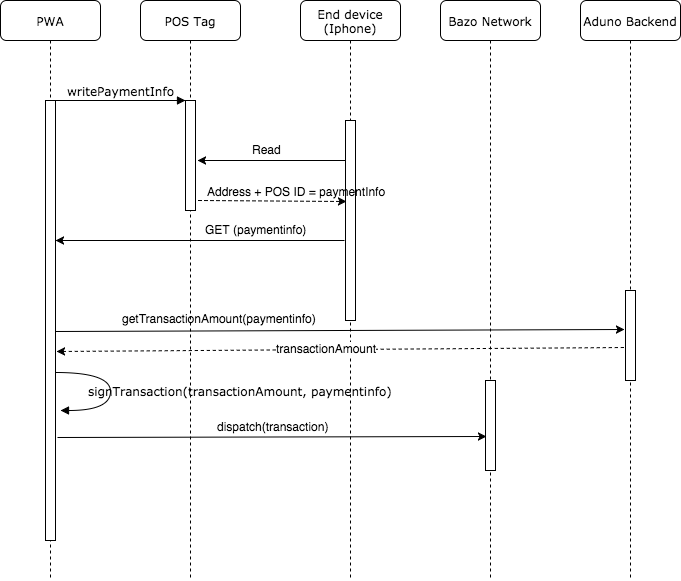
\includegraphics[width=1\textwidth]{diagrams/POS_flow.png}
\caption{\label{fig:POS}Payment process using an NFC tag with static transaction data.}
\end{figure}

\subsection{Onboarding Process and Account Generation}\label{onboarding}
This chapter describes the design of the process how a new account can be created and how an existing account can be topped up with Bazo coins.
Initially, a user would have to use the Bazo Wallet to generate a new ECDSA key pair consisting of private and public key. This key pair is not considered as valid account, where an inbound transaction could be executed on the account. This approach differs from other cryptocurrencies such as Ethereum \cite{myethwallet}. The reasoning behind this difference lies in the design of the Bazo currency, which is intentionally private. This means, that a key pair is only then a valid account if an \textit{AccTx} is executed. The registration of a public key therefore requires a transaction containing the public key of the new and root account. This transaction would then be signed with the private Key of the root account.
Assigning new funds to a registered account requires that the financial service provider deducts the bonus points from the user and sends a \textit{FundsTx} to the users public key. In order to determine if a user may participate in the program and to deduct the bonus points from the correct account, the user needs to manually obtain a token, which is then sent with each request.


\begin{figure}
\centering
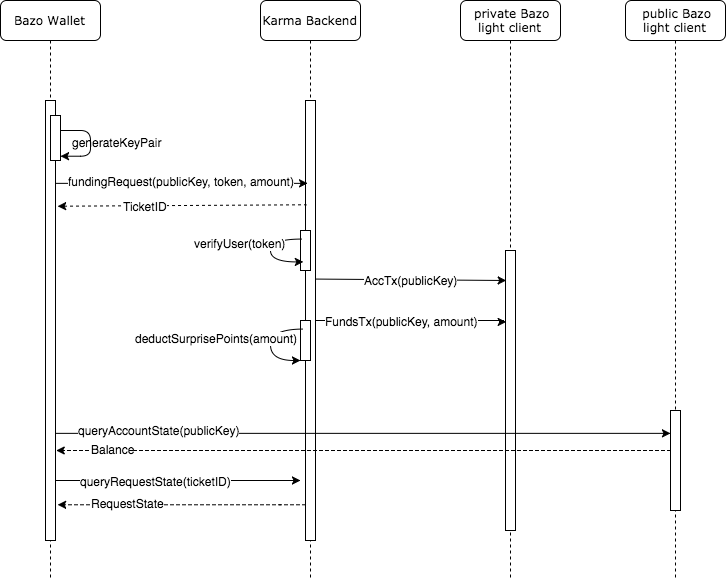
\includegraphics[width=1\textwidth]{diagrams/onboarding.png}
\caption{\label{fig:onboarding}Process of generating and registrating a new account.}
\end{figure}

\begin{figure}
\centering
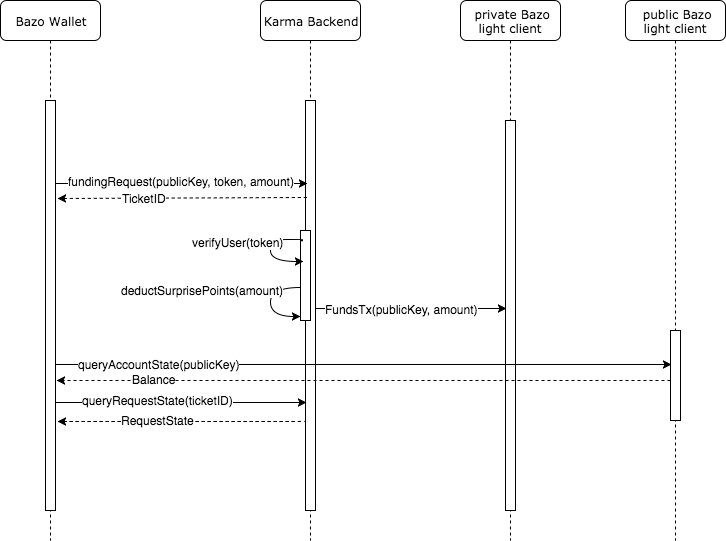
\includegraphics[width=1\textwidth]{diagrams/topup.png}
\caption{\label{fig:topup}Process of requesting new Funds for an existing account.}
\end{figure}



\chapter{Implementation}
Chapter \ref{design} introduced the design of the Bazo Wallet in order to fulfill the requirements to such an application documented in Chapter \ref{requirements}. This Chapter documents the implementation phase of the application. Chapter  \ref{architecture} outlines the architecture, the application employed. The following sections explain how the individual functional requirements were implemented.
\section{Architecture\label{architecture}}
The application was implemented as a Progressive Web Application. The characteristics of a progressive web application have been outlined in Chapter \ref{pwacharacteristics}. The application was implemented as a web application with the addition of the following items to comply as a progressive web application:
\begin{itemize}
\item Manifest
A manifest is a JSON file that describes metadata of a web application such as links to icons for different screen sizes. It is further used to configure the progressive web application. For example, the name that will be displayed in the app drawer on the phone once the app is installed, can be set here. It is important to note that only Google Chrome on Android supports manifest files. \cite{manifest} Other platforms, such as iOS rely on meta tags in the main html file of the web application \cite{applemetatags}. Implementing meta tags and manifest was straight forward, the names and description of the application had to be given, and the static ressources such as icons had to be linked correctly.
\item Service worker and Offline Capability
A service worker is a method to enable background processing of certain actions. A common way how service workers are used is to enable offline capability by intercepting web requests. By caching static parts of the web application, offline availability is enabled \cite{serviceworkers}. The service worker used in the project is automatically generated at compile time by a webpack plugin. This makes it possible to flexibly configure the service worker and define all the static resources which are then cached for offline usage. The offline experience is further enhanced by an event listener, which is integrated in the routing of the SPA. If a user is on a page that requires network access, the application will then inform the user about the network loss and redirect to the Home page.

\item Security Constraints
User-agents such as Google Chrome pose certain security constraints to allow a web application to be installable. This restricts web application and all cross-origin requests to be in a secure context, such as secured http or websockets \cite{manifest} \cite{securitychrome}.
\end{itemize}

\subsection{User Interface}\label{userinterface}
The application was implemented as a Single-Page-Application. With SPAs, it is possible to structure content and application interface into pages without leaving the document. %find sources%, 
This deals with the quality requirement, that the application should run in the browser with as little logic on the backend as possible. The Wallet was structured into the following pages, each accessible through a unique URI, although all technically in the same document:
\begin{itemize}
\item \textbf{Home Page}
This is where the user will be directed upon loading the application. If a user tries to access a page, he is not allowed to, he will be directed to this page. For example, if a user opens the link to the payment page of the application, but the network connection is lost, he will be temporarily be redirected to the home page until network access becomes available again.
\item \textbf{Settings Page}
On this page, the user can edit configurations such as showing or hiding advanced options on the other pages, which are directed at users in the role of a merchant. This would mean that the user has an additional field available to encode the POS ID into the transaction data. Further, the user is given the possibility to set the URI of a Bazo client web interface, that is then used for further communication with the client's web interface.
\item \textbf{Accounts Page}
Whenever a user tries to access any of the other pages except for the Home and Settings Page, without an account being stored in the browser, he will be redirected to the accounts page. Here, it is possible to store new Bazo accounts, by supplying the public key and a name to identify the account. Every public key can only be stored once, so that the total balance can be computed from the set of accounts. All accounts stored in the browser are displayed in a table, along with information such as balance, name and address for every account. Each of the stored accounts can be inspected in the Bazo Block Explorer, see \ref{bazoblockexplorer} and deleted from the storage. An account can also be selected to be the main account used. This account will then automatically get preselected for all other operations on other pages.
This page can also be opened with an address supplied in the URI, which would then be filled into the form. This is employed to make the process of inviting the user into the system easier.
\item \textbf{Requesting Funds Page}
When a user wants to share transaction data with another user, he would use this page. Here the user can set the necessary information such as target address and transaction value. If the user has selected advanced options in the Settings Page, he may set an identifier for a POS system. 
The compiled transaction data can then be transferred to other users using as many of the transaction sharing methods, as supported by his device and browser. Only the sharing methods supported by the underlying platform are visible to the user, in order to progressively enhance the application. For each of the transfer methods, an overlay would be opened to instruct the transfer process and to indicate the state of the transfer.
\item \textbf{Sending Funds Page}
If a user opens transaction data which is encoded into a single URI, he would be taken to the Sending Funds Page.
All transaction data supplied as parameters in the URI are then parsed and filled into the form. If a POS id is present, see \ref{transactioninfo}, the transaction value is looked up. All of these informations can also be manually supplied by filling out the form. In either cases, the user needs to select an account from which he wants to deduct the transaction, given that multiple accounts are stored. For said source account, the maximal amount of coins to be spent is displayed on the page. If the transaction data is valid, the user can request the transaction to be initiated. Once the transaction is prepared, a modal is opened, where the user needs to enter his private key, which is used to sign the transaction. The process of preparing, signing and submitting a transactoin is further described in \ref{blockchaininteraction}.
\item \textbf{Obtaining new funds}
This page allows users to inspect and submit new requests to deduct value from the bonus program and to top up a supplied Bazo account.
The user interface consists of table, where previous fund requests are displayed along with their state, and a form to submit new requests. The user has the possibility to generate a new account to select as a recipient for the coins. In order to make a new request, the user needs to supply their token, target Bazo address and the amount of coins he wants to receive. 
\end{itemize}
The described pages are always a standalone display, where it is not possible for a user to be on multiple pages. However, there are parts of the User Interface that are shown on all of the pages. These parts along with the individual pages were logically structured into reusable components:
\begin{itemize}
\item \textbf{Navigation Bar}
The navigation bar, which is located at the top of the screen holds multiple items. The icon of the project, a display of the total balance over all accounts and the currently selected main account are displayed. 
On devices which are less than 550 pixels wide, the total balance and main account are hidden.
\item \textbf{Side Bar}
The side bar is located at the right side of the document and can be used to navigate between the individual pages. If there is no account configured in the application, only the Settings and Account pages are shown. If there is no network access, navigating between pages is restricted to the Home, Settings, Accounts and Requesting Funds pages.
The sidebar also contains a display of the total amount of balances over all accounts and the icon of the project. Users can select between German and English languages at the bottom of the Sidebar. Each text in the application is fully internationalized in these two languages.


\item \textbf{Offline status display}
There is a background service, which is constantly checking if the application has network access. If this is not the case, the usage of the application is restricted to the Home, Settings, Accounts and Requesting Funds pages. If a user happens to be on any other page during connection loss, he is taken to the Home page where the Offline status display is shown. If the user does not navigate further he will be taken back to the original page, once network connection is obtained again.
\item \textbf{Progress Bar}
On each of the pages there is a thin progress bar at the very top of the document, above the header. This progress bar is used to indicate the progress of network requests made after the application is loaded.

\end{itemize}

Since the User Interface of the coinblesk-frontend application was structured as a SPA with reusable components, it was possible to use this application as a base \cite{coinbleskfrontend}. Since that application was designed as a client-server application, most of the logic had to be rewritten. However, it was possible to inherit the application structure as well as certain components. The Home Page as well as the four components that are visible on all pages were reused. Few modifications such as styling had to be applied. Almost all individual pages had to be rewritten. When doing this, the same User Interface Framework was used, since it provided reusable components and a consistent look with other parts of the application. A webpack configuration was used to optimize and build the application.

\begin{figure}
\centering
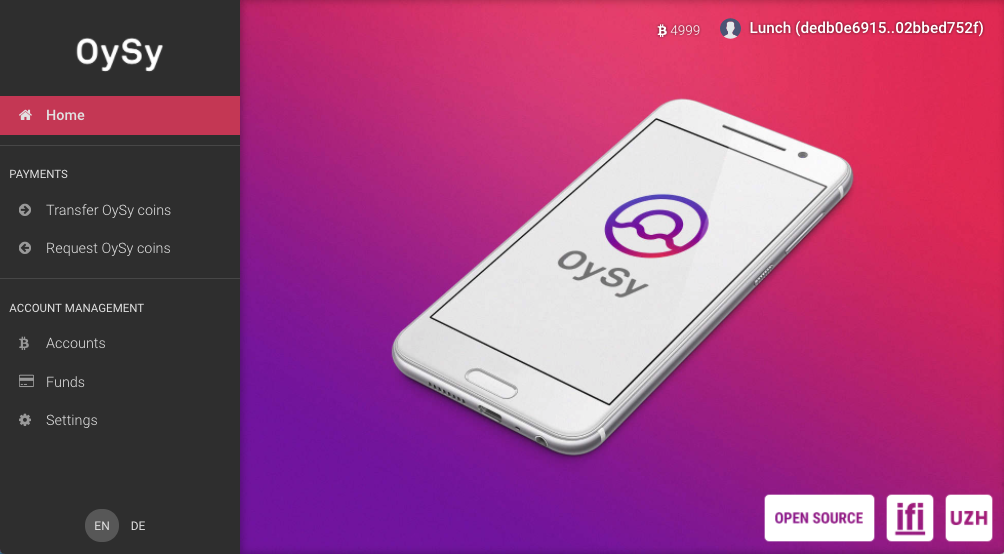
\includegraphics[width=1\textwidth]{screenshots/Home.png}
\caption{\label{fig:uihome}Home Page with Side Bar and Navigation Bar on a Desktop Device.}
\end{figure}

\begin{figure}
\centering
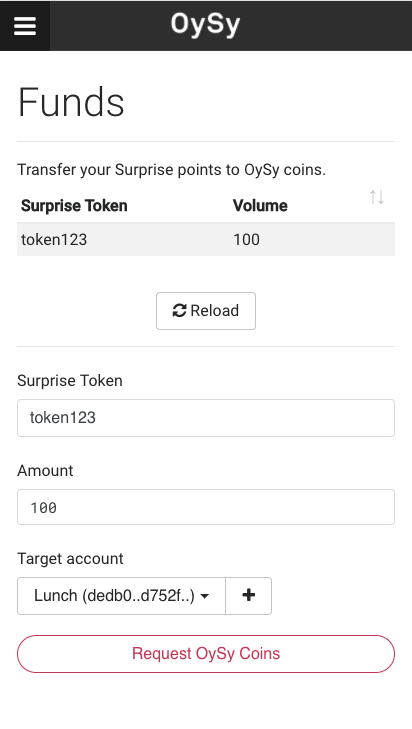
\includegraphics[width=0.75\textwidth]{screenshots/Funds-1.png}
\caption{\label{fig:uifunds1}Funds Page: Inspect and create new funding requests from bonus points.}
\end{figure}

\begin{figure}
\centering
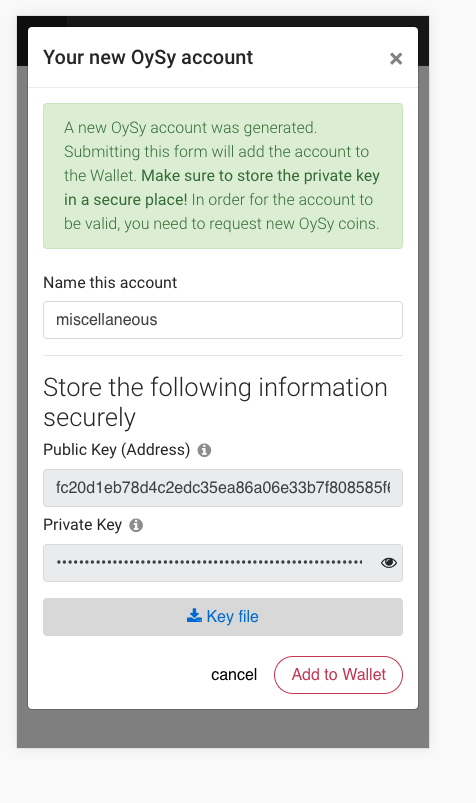
\includegraphics[width=0.75\textwidth]{screenshots/Funds-2.png}
\caption{\label{fig:uifunds2}Funds Page: Generate, save and export a new Bazo account for new Funding requests.}
\end{figure}

\begin{figure}
\centering
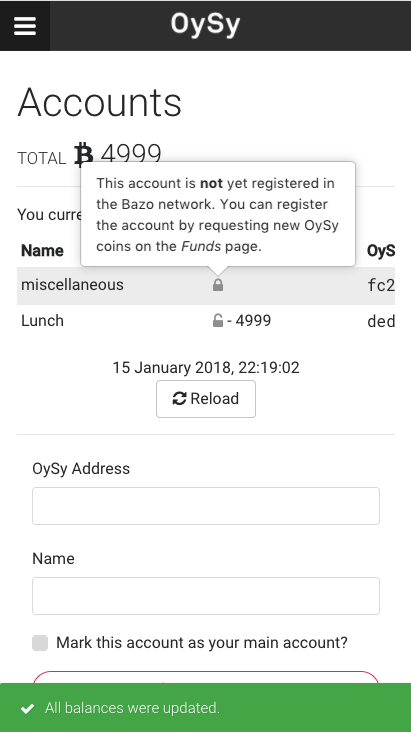
\includegraphics[width=0.75\textwidth]{screenshots/Accounts.png}
\caption{\label{fig:uiaccounts}Accounts Page: Add and inspect existing Bazo accounts.}
\end{figure}

\begin{figure}
\centering
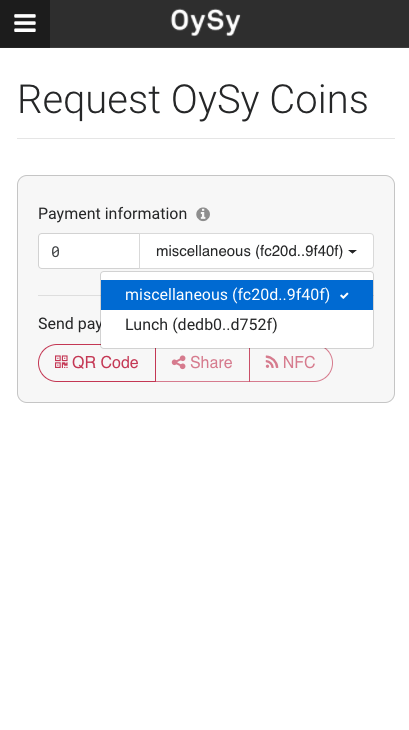
\includegraphics[width=0.75\textwidth]{screenshots/Request-1.png}
\caption{\label{fig:uirequest1}Request Page: Compile shareable payment information.}
\end{figure}

\begin{figure}
\centering
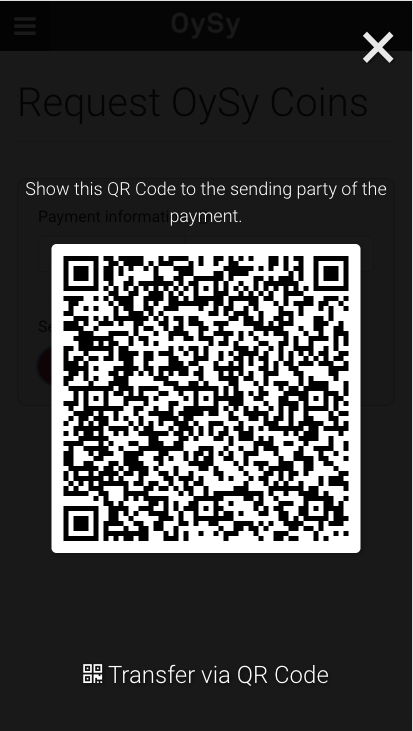
\includegraphics[width=0.75\textwidth]{screenshots/Request-2.png}
\caption{\label{fig:uirequest1}Request Page: Transfer payment information with one of the transfer methods.}
\end{figure}

\begin{figure}
\centering
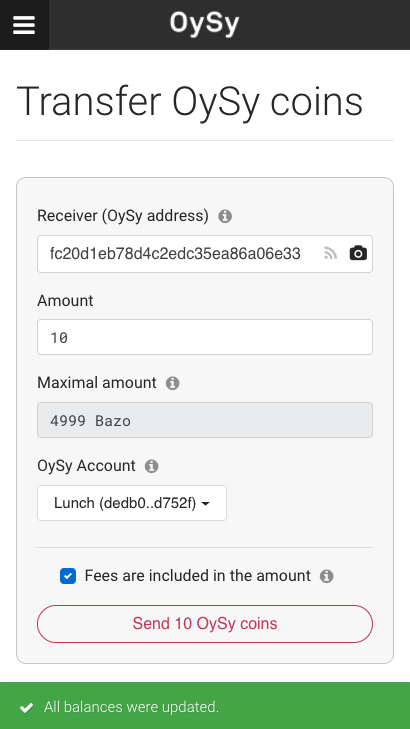
\includegraphics[width=0.75\textwidth]{screenshots/Send-1.png}
\caption{\label{fig:uisend1}Send Page: Fill in payment information or receive them through one of the transfer methods.}
\end{figure}

\begin{figure}
\centering
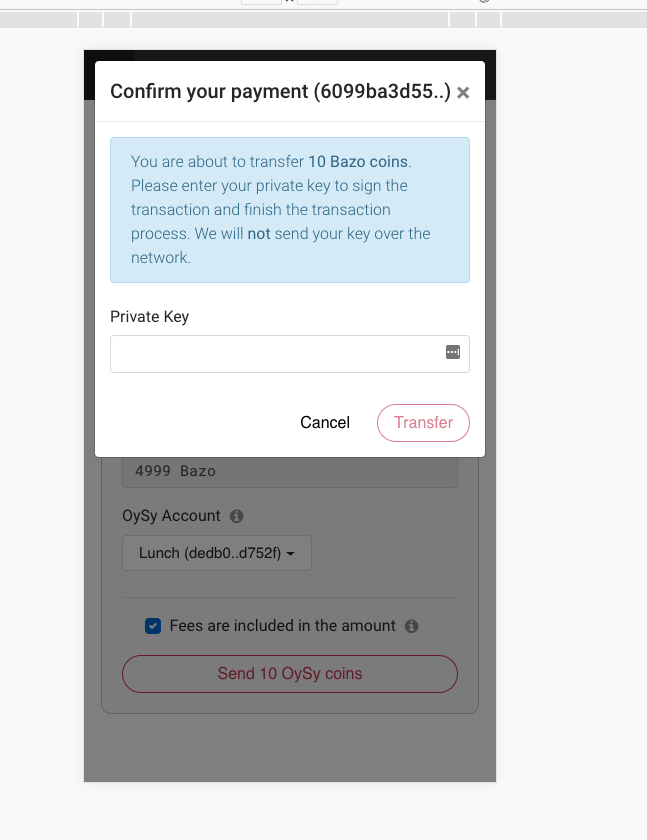
\includegraphics[width=0.75\textwidth]{screenshots/Send-2.png}
\caption{\label{fig:uisend2}Send Page: Confirm and sign the payment.}
\end{figure}

\begin{figure}
\centering
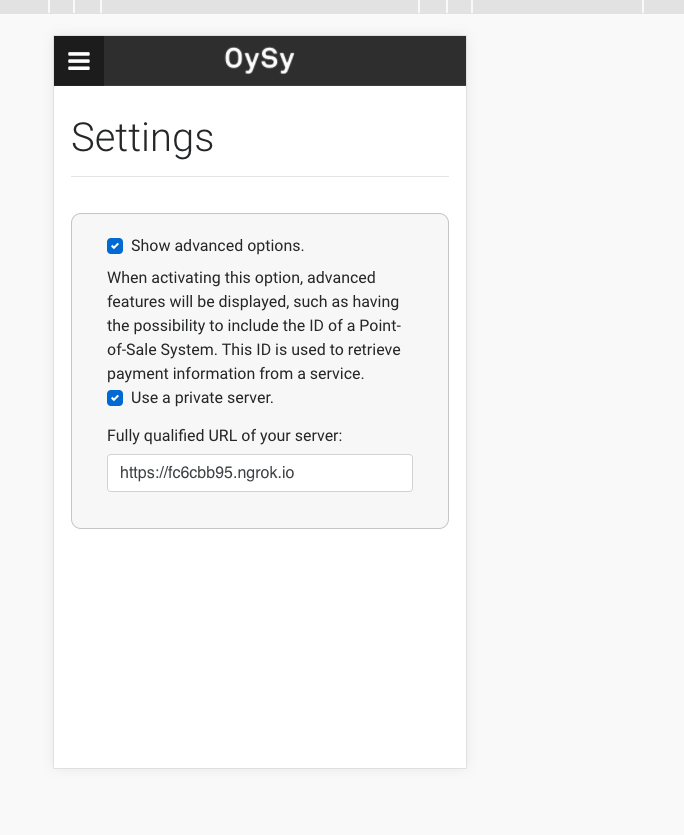
\includegraphics[width=0.75\textwidth]{screenshots/Settings.png}
\caption{\label{fig:uisettings}Settings Page in the Bazo Wallet.}
\end{figure}


\subsection{Storage and State management\label{storageandstate}}
In Chapter \ref{qualityrequirements}, the requirement for complete client-side operation and security requirements were introduced. This implied, that a storage solution local to the browser had to be used. HTML5 Web Storage is a browser side storage solution, that is supported by the majority of browsers \cite{localstoragetest} \cite{localstorage}.
%part?%
In the Security part of the specification document, multiple issues with the security of Web Storage are explained \cite{localstorage}.
With a new API for browser side encryption in discussion by the World Wide Web Consortium, mechanisms like symmetrically encrypting values in the storage could be leveraged. However, the API is only considered a Recommendation of the Consortium\cite{webcrypto}.
This makes local storage of security related data such as private keys unsuitable. Therefore, only user-data such as settings and public keys of Bazo accounts were stored in the Web Storage. For explicit state management vuex, a library for state management with Vue.js was used \cite{vuex}. The subset of state that needed to be persisted in Web Storage was placed in this storage.
%??%
\subsection{Network Communication}
Multiple operations of the Bazo Wallet are performed using cross-origin http requests. These operations include payment preparation, payment submission and account balance querying. All of these operations are centralized in a single Service module, that can be shared between the individual components. With this it is possible to parametrize network requests globally. This is a requirement, so that the URI used to perform the requests can be configured by the user. The actual communication with the endpoints of the Bazo client and their semantics are explained in \ref{blockchaininteraction}.

\section{Transaction Sharing}
Requesting payments is a core requirement for the Bazo Wallet to qualify as a payment system for end-users. The design of the sharing process and the data model were explained in \ref{transactioninfo} This section explains how sharing transaction data across devices was implemented.
\subsection{Web APIs and Browser Support}\label{browsersupport}
At the time of writing, more and more native API's are made available for the Web.
However, the API specification for NFC connectivity in the browser is still in draft \cite{webnfc}. Partial implementations of the API are available in Google Chrome on android devices. Other user-agents and platforms do not yet support the feature although some have expressed intent to implement. The implementation state in Google Chrome is not documented thoroughly since there exists no implementation report yet, as they are available for other specifications \cite{localstoragetest}\cite{webnfc}. This implied that the specification and Google Chrome's source code was the only way to obtain information on the subject apart from testing.
% TODO Reference state for Webkit, moz, IE.
For the prototype, the feature was implemented for Google Chrome on android.
In order to allow web-nfc in Google Chrome, there need to be two flags set to enable the experimental implementation: \textit{Experimental Web Platform features} and \textit{webnfc}. The first of these flags will show the nfc object in the navigator object of the browser. However, this does not mean that the hardware does support web-nfc. The latter flag can only be set on devices whose hardware actually supports NFC. This approach of hiding functionalities behind flags to let developers test the implementations, are called origin trials, in the Chromium Projects \cite{origintrials}.
After extensive testing, it became clear that the current implementation of Google Chrome only allows devices to use NFC functionalities such as reading and writing to NFC tags as a target. Performing these actions to active NFC devices such as a smartphone will throw the corresponding error according to the specification draft \cite{webnfc}. After discussion with members on the working group, they confirmed that targeting active NFC devices is not yet implemented. The reason for this is that these operations would require native UI elements from the android operating system. However, they expressed intent on implementing it in the future \cite{webnfcpeer}.

Another challenge posed the creation and signing of Bazo transactions in the browser. The structure of a Funds Transaction can be seen in figure \ref{fig:FundsTX}. Since not all data-types that are usually available in C-like structs, are available in the browser, a bridging solution had to be implemented. The application was therefore designed as a signing-only client, with the implication of designing a web interface into the light client as described in \ref{networkandinterfaces}. This is a common approach when building web based Wallets that don't store the users private key on a server \cite{bitcoinclients}\cite{masteringbitcoin}.

\begin{algorithm}
\caption{FundsTx}
\label{euclid}
\begin{algorithmic}[1]
\State type FundsTx struct $\{$
\State \ \ \ \ Header byte
\State \ \ \ \ Amount uint64
\State \ \ \ \ Fee uint64
\State \ \ \ \ TxCnt uint32
\State \ \ \ \ From [32] byte
\State \ \ \ \ To [32] byte
\State \ \ \ \ Sig [64] byte
\State  $\};$
\end{algorithmic}
\end{algorithm}\label{fig:FundsTX}Structure of a FundsTx in Bazo \cite{lisg}.

%%\begin{figure}
%%\centering
%%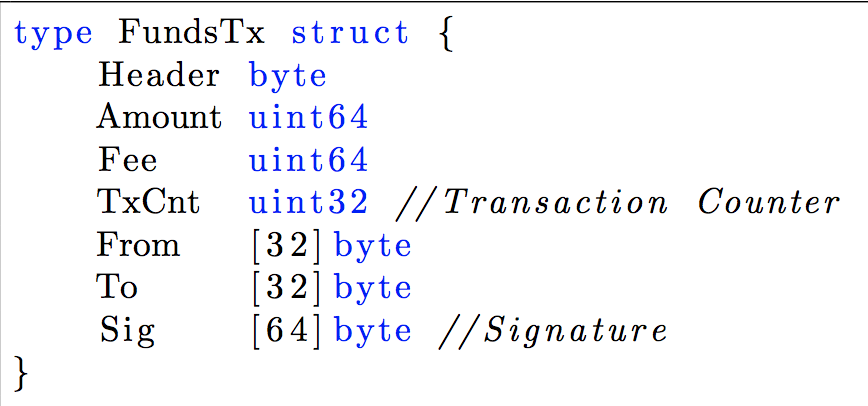
\includegraphics[width=1\textwidth]{diagrams/AccountTx_struct.png}
%%\caption{\label{fig:FundsTX}Structure of a FundsTx in Bazo \cite{lisg}.}
%%\end{figure}

\subsection{Web NFC}
In section \ref{pocnfcbridge} the semantics of the data model of a transaction that can be shared among users in the form of a single URI was explained.

NFC also enables devices to share information at a distance that is less than 10 centimeters. Users can share business cards, make transactions, access information from a smart poster or provide credentials for access control systems with a simple touch.
NFC, is a technology standard that allows contactless, two-way data transfers between devices that are within centimeters of distance \cite{nfcforum}.
Since the support for WebNFC is limited to android devices, the functionality for writing and reading the transaction data is visible only to the users that have activated advanced options.
The corresponding UI elements are therefore hidden if the user has not activated advanced options. The same goes for browsers and devices that lack webnfc or nfc support.
Using the API for the actual read and write operations was straightforward since the API consists of one method for each of them. The data type of the NFC record was set to URL.
This way the URI can be read from all types of devices. Android devices can therefore use the android system or the Bazo Wallet to scan the Tag. If the android system is used, the tag can be placed to the back of the device. If NFC is activated in the system settings and the user has unlocked the phone, the NFC record is parsed. Since the data type of the NFC record is a single URI, android's intent system is used to ask the user which application to use for the URI. This should include Google Chrome for all standard installations and the Bazo Wallet itself, if it is installed to the homescreen.


\subsection{NFC Bridge}\label{nfcbridge}
Due to limited browser support for Native API's such as webNFC, see \ref{browsersupport}, a prototype was discussed and implemented in the scope of this thesis. The prototype involved a native android application that should enable the web application to forward transaction information that could be forwarded to NFC capable devices using the Android Beam technology.
The design and requirements of such an application was outlined in \ref{pocnfcbridge} and the two main functional requirements for the application were presented.
Reading NFC messages from passive and active devices, was achieved without implementing it in the android application. This was done by changing the data model for transaction information to one that can be expressed in a single URI. With this media type, it is possible to use the tag dispatching system in android. This would work as follows:
\begin{enumerate}
\item An NDEF message is received when the android device is unlocked and NFC enabled.
\item The NDEF message for this application contains just a signle URI. Through android's intent system the application that fits best is started.
\item If the Bazo Wallet PWA was previously installed on the android device, an intent filter is present for the origin URI of the PWA. This will result in the PWA being opened with all transaction data passed as parameter.
\item If the Bazo Wallet PWA is not installed there will be no intent filter requesting the data. The user is then prompted with all applications that can handle an URI, such as a Web browser. If a browser is selected, then the Bazo payment page is opened with all transaction data passed as a parameter.
\end{enumerate}

%https://developer.android.com/guide/topics/connectivity/nfc/nfc.html

Writing the transaction data to other android devices was implemented using the Android Beam technology.
The transaction data can be passed to the NFC Bridge by either manually entering it into a form or by passing it as data through an intent. Passing data to the application through parameters has the benefit that web applications can generate links that will take the user to the application. Such a link can contain further data, which would be set to the transaction data the user wants to share with another android device.
If the android phone is held against another Android Beam enabled device, the NFC Bridge application will automatically set the appropriate transaction data encoded as an NDEF message and push it to the other device.

At the time of writing, NFC support for iOS platforms was just released for their most recent publicly available version, iOS 11. The NFC functionality offered to iOS developers covered writing and reading to NFC tags on the iPhone 7 and iPhone 7 Plus \cite{corenfc}. Thus, an NFC Bridge application similar to how it was developed for android would not extend the functionality of existing generic NFC applications. The NFC fallback capabilities with the Bazo Wallet on iOS are outlined in Chapter \ref{fallback}.
\subsection{Bluetooth Low Energy}\label{ble}
Bluetooth Low Energy, allows for devices to exchange data in short wireless connection. Devices will usually establish connections in a peer-to-peer topology \cite{blep2p}. Data can be structured into GATT-services which is then exposed to other BLE-capable devices. These devices may then perform actions such as reading and writing on these Services \cite{blegatt}. 
This makes the web-bluetooth API useful for web applications interacting with BLE-devices in proximity. However, to use the API for transaction sharing between two web pages on different devices, this would imply for one of the devices to take on the role of a server. This functionality is not provided in the web-bluetooth API, and makes it therefore not suitable to solve the requirement \cite{webble}. 
%%This was confirmed by \cite{undefined}.

Since the web-bluetooth API could not be used for data sharing, the websharing API was leveraged to provide easy sharing capabilites with low friction. Low friction for usage is given through the deep integration of the API with android's intent system. By invoking the API through passing the relevant URI, all sharing options available to the device will be presented to the user \cite{webshareapi}. This has two advantages:
\begin{enumerate}
\item Technologies such as Bluetooth, E-mail, SMS and even Android Beam are always available, even on system without installed third-party applications.
\item Sharing transaction data is not limited to functionalities provided by the Wallet. The user has the possibility to use any existing application, for example, his favorite chat applicatoin, to transfer the URI. When new applications are installed, they are automatically registerend and then considered by the android's intent system for sharing.
\end{enumerate}

The Web Share API is not considered a W3C standard, however it was assessed as an origin trial in Google Chrome on Android and is now normally available starting with version 61 \cite{webshareapi}\cite{websharespec}.


\subsection{Quick Response Codes}\label{qrcodes}
Quick Response Codes were initially envisioned to be the fallback way to transfer transaction data for devices that either do not support NFC or in cases where the browser does not support webNFC. With the data model explained in \ref{schema}, all transaction data can be placed in a QR Code in the form of a single URI.
This data model was chosen with the intent to support devices where the browser does not allow camera access in the browser over the webRTC API, which is still not widely adapted by browsers \cite{webrtcimplreport}. Testing Google Chrome and Safari on desktop and mobile systems showed that only Google Chrome has implemented the webRTC API for camera access. Safari has  implemented webRTC into their most recent version 11, which was released to the public in September 2017  \cite{safari11release}\cite{ios11release}. This implies that users with older versions of iOS will not have access to the API. Users with such a device can still read the QR Code using a generic native application. Since all information is encoded in a single URI the payment page can be opened with all necessary information prefilled.
Google Chrome has already implemented the webRTC API, therefore multiple QR Reader libraries leveraging the API exist.
The QR Scanner from the coinblesk-frontend project was a simple wrapper around an existing QR Reader library \cite{instascan}. Due to the implementations in Safari version 11, the underlying library had to be modified so that certain attributes were set. This allowed to run the QR Reader in the Browser of iOS devices. The actual decoding of the image with the library is implemented in pure JavaScript. This has performance drawbacks, since there is no hardware support. Further, the library is quite large with around 1.5 MB size for a minified JavaScript file. Because of this, the ShapeDetectionAPI was evaluated, which promises certain optimizations, since the decoding is not run in JavaScript \cite{shapeapinotes}. However, this new API is neither a W3c Standard or on track of becoming one \cite{shapeapispec}.

\subsection{Fallback Solutions}\label{fallback}
Subsections of Chapter 4.2 outlined how existing native and web-enabled API's were leveraged for the Bazo Wallet to share transaction data. This section documents the fallback solutions that were evaluated for devices or platforms that lack the support for the API, either natively or on the web.
For android, the complete functionality of NFC could be leveraged. Writing and reading NFC tags was implemented with the web-nfc API. Complete peer to peer communication was enabled by developing an API bridge, see \ref{nfcbridge}. A similar functionality is also provided by the webshareAPI implemented for Bluetooth transferrals \ref{ble}.
As iOS platforms only support native API's when communicating over NFC and peer to peer mode is not yet included, the fallback solution to use NFC on iOS consists of using a native application. Writing the NFC tag can be done with any generic NFC application or, on an android device, with the Bazo Wallet itself.
Initially a QR-Code was envisioned to be the fallback solution that should cover all devices. However, reading a camera video stream is only possible for the most recent version of iOS. This implies that this can not be used as a fallback solution for older iOS devices, although the same procedure as with NFC, where an existing native application can be used for scanning is possible.
Because of this limitation in iOS, a solution where the URI with all transaction data is being copied to the users clipboard was implemented for both systems. This way, iOS users have a convenient way of obtaining the URI and can then manually distribute the URI over their preferred channel. The same functionality is offered to android users over the webshare API which has a better integration into the android system, so that the URI is directly passed to the androids intent system for sharing, see \ref{ble}.

\section{Blockchain Interaction}\label{blockchaininteraction}
Actual network communication with the Bazo network in a trustless way posed the most difficult technical challenge for the application. The following operations and issues had to be evaluated:

\begin{enumerate}
\item Building the transaction data in the schema defined in the Bazo protocol. \ref{fig:FundsTX}.
Due to technical limitations of the browser, this application context is not suitable to fulfill the requirements of a light client implementation. Reasons for this are lack of support for tcp communcation, appropriate storage solutions and data structures.

\item Signing the transaction data with the appropriate algorithms.
\item Verifying transaction and account information.
In order to run the Bazo Wallet as trustless as possible, the application has to maintain at least a certain amount of the blockchain to verify information. For the Bazo Wallet this would mean that the Bazo Wallet itself needs to verify blocks and transactions, or that the Bazo Wallet needs to communicate with a trustworthy Bazo client. 
\end{enumerate}
% link to gomobile, link to evaluation & future work


\subsection{Bazo Client Web interface} \label{bazoclientwebinterface}
In order to interact with the Bazo Client, a web interface had to be created. The web service was designed as a RESTful API and implemented into the light client.
The web service consisted of two endpoints for each type of transaction in the Bazo currency and one for the retrieval of account information such as balance and other parameters.
For each of the transaction types the following two endpoints need to be used.
\begin{itemize}
\item The endpoint at /create<Account Type>/ is used to create and obtain a transaction hash given all parameters for the Transaction struct are sent. This solves the problem of lacking the appropriate data types in the browser. The  returned transaction hash can then be signed on the client.
\item The endpoint at /send<Account Type>/ accepts the transaction signature, which was generated on the client, and matching transaction hash. With these informations, the transaction can be considered complete, so that the underlying Bazo client can distribute the transaction for further validation in the network. The web service does not validate the transaction and respond the answer to the client.
\end{itemize}  

\subsection{Transaction Signing}\label{transactionsigning}
Due to limitations of the browser for C-like structures as they would be required to create a FundsTx, an interface had to the Bazo client was to be developed. 
The process of obtaining transaction information, requesting a new transaction, signing and dispatching it into the network is shown in figure \ref{fig:TransactionProcess}. The process can be described as follows:
\begin{enumerate}
\item The application queries the necessary account information to request a transaction struct in a later step. This is a necessary step, since the TxCount of the transaction has to be correct in order for the transaction to be valid.
\item When the account information is read, the web application can send a request to the web service to create a new FundsTx struct. The Bazo client creates the appropriate structure, hashes it using the \textit{SHA3-256} algorithm and returns it to the Wallet.
\item The Wallet is now in charge of asking the user about its private key and signing the received transaction hash, using the \textit{ECDSA} algorithm on the \textit{p256} curve. The resulting signature and transaction hash pair then needs to be sent back to the Bazo client for distribution in the network.
\end{enumerate}

This approach is comparable to the mechanism employed in the official JavaScript API of the Ripple currency \cite{ripplelib}.
Figure \ref{fig:ripplesendTx} demonstrates how a transaction can be sent with the Ripple cryptocurrency using the official library. The mechanism can be outlined as follows:
\begin{enumerate}
\item A connection to an interface is opened over a Websocket. 
\item A request is made to obtain relevant data and instruction for the payment.
\item The data returned from preparing the transaction is signed.
\item The API submits the signed Transaction over the WebSocket.
\end{enumerate}


Comparing the mechanism in Bazo, see Figure \ref{fig:TransactionProcess}, and Ripple, \ref{fig:ripplesendTx}, reveals certain differences, although the approach, with the respective consequences being similar.
\begin{itemize}
\item \textbf{Protocol mechanism} In Ripple, there exists a convenient method to prepare all data into a single JSON object, that needs to be signed and submitted. This step is splitted up into multiple steps in the web interface for Bazo. The client is responsible for querying the account information and then requesting a transaction hash from said information.
\item \textbf{Connection Type} Both cryptocurrencies use web interfaces for communication with a node in the Network. In Bazo http is used, while the Ripple library makes use of a WebSocket for two-way communication. Given that two-way communication is not necessary for the Bazo currency, the http approach was chosen, since this is supported by a broad range of devices and browsers.
\end{itemize}

\begin{figure}
\centering
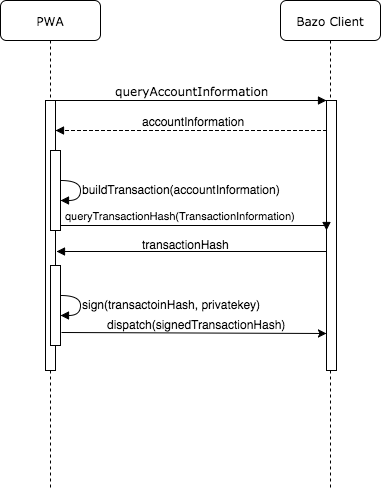
\includegraphics[width=0.7\textwidth]{diagrams/transactionProcess.png}
\caption{\label{fig:TransactionProcess}Requesting, building, signing and submitting payment information with the Bazo Wallet.}
\end{figure}

\begin{figure}
\centering
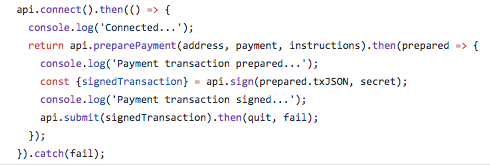
\includegraphics[width=0.7\textwidth]{diagrams/ripplelibSendTX.png}
\caption{\label{fig:ripplesendTx}Programmatically creating, signing and sending a transaction with Ripple-lib \cite{ripplelib}.}
\end{figure}


\subsection{Client Integration}\label{bazomobile}

Chapter \ref{bazoclientwebinterface} explained the interaction between the Bazo Wallet and the Bazo light client over a web interface.
This Chapter explains contexts in which the Bazo client can be run, consequences and documents the efforts of porting the light client to mobile devices.
Due to the security constraints one needs to consider when interacting with cross-origin resources in a PWA, the Bazo client web interface has to be in a secure context \cite{securitychrome}. This would mean that an SSL certificate needs to be installed or that the server needs to accessible through a secure reverse tunnel.
This makes mobile devices as a runtime difficult. However, a proof of concept was developed to show that mobile devices are technically feasible to run the client. 

To overcome these limitations, native application wrappers for the light client written in Go were evaluated. 

The first approach for porting the light client, which was written in the \textit{Go language}, evaluated the usage of go bindings for java. These could then be used in a native Android application. There exists a project \textit{go mobile}, that can be used to generate bindings from a package written in \textit{Go}. However, the current state of the go mobile project did not support all networking and data structure needs to fulfill the requirement. Further, this would have required to restructure the go application as a package \cite{gobind}. Programming to such bindings usually has the advantage, that the Java application can directly call methods of the binded package. Since all communication between the actual Wallet application would go over the http interface, this would not pose an advantage.
The second approach focused on cross-compiling the Bazo client for the android operating system running on ARMv5 architectures.
To port the complete Bazo client without any modifications to the android operating system the application was compiled using the clang compiler. The compiler can be obtained through androids official NDK or it can be compiled from scratch. The complete toolchain was compiled targeting the arm architecture, and android API version 21 for a darwin x64bit system which was the host for the compilation \cite{standalonetoolchain}. The clang compiler of the toolchain was then used to configure the go environment for cross-compilation. This involved configuring the golang environment for arm architectures and to use the freshly compiled clang compiler \cite{gobuild}.
The binary was then copied to an android device an ran in the scope of an existing application. This is a necessary step for binaries that are run on devices were root access is not given. The application performed well, so that ngrok was used to create a secure reverse tunnel. With this in place the web application was able to interact with the Bazo client running on the same device but accessible through the secure context. Detailed instructions for installation can be found in \ref{bazoandroid}.
This Proof of Concept could be leveraged to create an actual android application wrapping the binary. However, a solution to configure SSL appropriately would need to be found.
% reference in future work

\section{Optimizations and Testing}
In order to assess and optimize the quality of the developed web application, Lighthouse was used for the audit. \begin{quote}
Lighthouse is an open-source, automated tool for improving the quality of web pages.
\end{quote}. 
There exist various workflows to run the tool, however, running it directly from the Google Chrome Developer Tools seemed the easiest. The audit can be performed against almost any web page, and assesses five key factors of web applications, such as \textit{Progressive Web App}, \textit{Performance}, \textit{Accessibility}, \textit{Best Practices} and \textit{SEO}. For each of the metrics, several audits are performed and then summarized to express the scoring as a percentage. It is possible to drill down and obtain detailed information on a failed audit. For some of the audits, the tool can even predict possible enhancements \cite{lighthouse}.
Running the tool against the deployed web application showed the strengths and weaknesses of the implementation. Initially, the application got the full score for \textit{Progressive Web App} and \textit{Accessibility}, which performs audits against the Progressive Web Application Checklist \cite{pwachecklist}. The biggest optimization potential was highlighted through the \textit{Performance} metric, which got a result of 44. There were various issues that hindered the performance of the application. These issues and their solution are explained in the following.
\begin{itemize}
\item Render-blocking scripts:

The JavaScript library that contained the decoder for QR-Codes, makes up a large part of the application's size. Loading the library from the start of the application had a negative impact on the loading time required until the application is drawn and interactive. This is an interesting fact, since the development of the Shape Detection API, introduced in \ref{qrcodes}, has the intention of avoiding the necessity to include a decoding library in the application. This issue was solved by dynamically loading the library, once the user enters the actual page where the decoding capability is needed.
\item Large images:

Images that are not properly sized, can also increase the loading time, thus affecting when the application becomes interactive. The images, supplied by the Design agency were compressed, resized and converted to a more suitable format to decrease the loading and rendering time. By doing so, the size of the assets was decreased by around 80\%.

\item Rendering time:

The time required to render the home page was further optimized by making use of a server-side rendering approach. Since the home page contains mostly static content, it was ideal for this technique. Server-side rendering was achieved by incorporating an optimization plugin into the \textit{webpack}-based build process.
\end{itemize}
The issues described above, led to initial loading times of around five to seven seconds until the application becomes responsive. It is important to note, that Lighthouse performs these tests under constrained settings. Network speeds are throttled to resemble mobile devices and caching is not leveraged. This testing environment is comparable to a mobile device with a slow network connection accessing the application for the first time. With the performance optimizations described above, the initial loading time was decreased under two seconds. Subsequent loading times would take around 250ms until the application becomes responsive, by leveraging the caching mechanisms.
After optimizing the application, the \textit{Performance} metric received a score of 77.

For the full score of the \textit{Best Practises} metric, the application would have to be deployed to a server that allows serving over HTTP/2. Since this is not part of the actual implementation of the web application and rather a question of deployment, this metric can not be improved with the code basis of the web application.

Lighthouse specifically proposes manual checks in order to ensure that the user experience is appropriate on multiple browsers and platforms. The same strategy is proposed for testing User Interfaces, with regard to page transitions and animations. 
Since the complete functionality with all branches can be relatively quickly tested, the complete app was tested for a variety of devices. The rest of this chapter gives insight into the testing results and the combinations of operating systems and browsers that have been tested.


\begin{center}
    \begin{tabular}{ | l | l | l | l | p{3cm} |}
    \hline
      & Internet Explorer & Google Chrome & Safari & Firefox \\ \hline
    macOS X (10.12.6)  & no & yes & yes & yes \\ \hline
    Windows 10 (14393.479)  & yes & yes & no & yes \\ \hline    
    iOS (11.1.2)  & no & no & yes & no \\ \hline
    Android (8.0.0)  & no & yes & no & yes \\ \hline
    \end{tabular}
    \captionof{table}{Combinations of browsers and operating systems where the Bazo Wallet was tested.}\label{table:testing}
    \end{center}
Table \ref{table:testing} shows targeted platforms where the complete functionality of the Bazo Wallet was tested. The web application proved to work as expected based on the evaluation of cross-browser support for the leveraged API's as described in \ref{browsersupport}. Testing the web application in Safari on an iOS device, revealed that there are still several issues with PWA's on iOS. First, the application behaves different, depending on if it is run directly from Safari or from the home screen. Given that WebKit, the browser engine used by Safari, still does not completely support PWA's explains the lack of stability. Many of the technologies used with PWA's, such as Service Workers are not completely implemented at the time of writing \cite{webkitsw}. However, using the web application in Safari provided a consistent user experience. All elements that require unsupported features were hidden from the user.
 

\begin{bclogo}[logo=\bcattention, couleurBarre=red, noborder=true, 
               couleur=LightSalmon]{Important!}
This section is incomplete. The content on testing is missing.
\end{bclogo}
\newpage


\chapter{Evaluation}
The ecosystem of the Bazo cryptocurrency can not be considered completed to a degree where a test run would be possible, at the time of writing. Reasons for this are that the development of the interfaces of the existing infrastructure was not completed. Since these interfaces were specifically designed for the Bazo Wallet during the course of this thesis, the Wallet itself can be considered complete. This chapter assesses the developed Wallet and explains limitations to the system.
\section{Prototype Evaluation}
This section evaluates the developed P2P mobile payment application against key characteristics for such a solution. Key characteristics of a mobile payment solution can be:
\begin{enumerate}
\item \textbf{Speed}
The speed of a payment is characterized as the time passed between initiation and clearance of the transaction.
\item \textbf{Payer control}
This refers to the degree as where a user can select the most advantageous terms for his payment.
\item \textbf{Security}
The degree of risk of having funds manipulated or stolen by engaging in the payment system is considered Security.
%inverse?%
\item \textbf{Universality}
This key characteristic deals with the importance of a payment system being accepted by a large user base to make the payment solution attractive.
\end{enumerate}

Considering speed, there are multiple issues for assessing the Speed of the Bazo Wallet. First, it is hard to determine where the start of the transaction process begins. It is assumed that the transaction process starts when the user has already all the necessary information such as target address and transaction value available. It is difficult to assess the speed of the Wallet since the speed of the payment depends on other systems. A high amount of unconfirmed transactions, a lower fee selected by the user and the configuration of the block interval can impact the payment speed. If we would assume these values were chosen optimally, the Bazo Wallet contributes little to no time to the overall time required for the payment. Obtaining transaction data, signing and submitting it from and to a remote Bazo client, took less than 500ms in tests. Using a local client, such as the Android version should require even less time, since most of the time is lost connecting to remote systems.

Payer control with the Bazo currency has a mixed image.
The user has the control to create transactions at terms he prefers, for example, the user can set the fee he is ready to spend for the transaction. However, the clearance of the transaction depends very much on the network. That is the current amount of unconfirmed transactions, the rate at which transactions are validated and the fee the user has set. The user has little to no influence on these conditions.

Security as in the definiton above, should be given for all transactions signed by the user. Section \ref{limitations} outlines cases, where the user can be tricked to reveal his public key. From a technical point of view, the Wallet can be considered secure, as that it is not possible to steal a private key or manipulate transactions which would result in the loss of funds for the user.

Universality is not a strength of the Bazo currency. Since the Wallet is not compatible with other payment systems or applications only users in the system can exchange funds. Since Bazo is a newly created cryptocurrency, there is no user base and users would have to be convinced to join the system. Given that the target users should already be in the bonus program, the usage of the Bazo currency could be offered an incentive. Since the mechanisms in the Wallet for communicating with the currency are very similar to the mechanisms in other currencies such as Ripple, it would technically be feasible to reuse the Wallet for other currencies and map the bonus points to said currency \cite{ripplelib}, thus leveraging an existing user base.

\section{Limitations}\label{limitations}
This chapter introduces limitations of the developed systems and how they can be improved.
\begin{itemize}
\item \textbf{Trust} 
It is an objective of many cryptocurrencies to be as independent from third parties as possible. This should that assets can be traded in a trustless way. Since, the application is designed as a signing-only client, there needs to exist a certain amount of trust between the user of such a Wallet and the server he relies on \cite{bitcoinclients}. With this architecture, it is technically possible to tamper with the information that is sent to the client, such as account balances. This is due to the client being unable to verify the transactions in the same manner that other applications can. However, it is not possible to modify outbound transactions and thus steal assets from the user of the developed system.
This is ensured by having all transaction signing implemented in the browser. Since sharing transaction data is not performed over the same server, but rather on a P2P basis, it is also hard to trick the user into targeting the wrong address.
Another solution how this threat can be reduced further is by giving users the freedom to connect to a specific server. In the Bazo Wallet, the user has the possibility to set a URL on the \textit{Settings} Page. This URL is persisted locally and used for all further communication. That way, users could deploy the light client to an https enabled server and use this node as a private backend. This approach is frequently employed when dealing with signing-only clients \cite{bitcoinclients}. It is also technically possible to run the light client locally on an android phone, by running the binaries of the light client. This was tested and proven to work as with any other operating system or platform.
\item \textbf{Phishing} 
Another risk is introduced with the unified data model of transaction data, since this points to the URL of the Bazo Wallet. One could trick a user into using a web application that looks like the Bazo Wallet, but has the single purpose of stealing the private key. This is a serious risk in cases where the user does not realize that the URI does not belong to the actual Wallet.
One solution how this weakness can be handled is to install the progressive web application to the home screen. On Android systems, this will associate the installed application with the URI of the origin. Therefore, the application will only open if the host of the URI matches the origin of the installed web page.
\item \textbf{Browser Support} 
Chapter \ref{transactoinsharing} assessed the support of different operating systems for new, web-based API's. Especially Safari on iOS devices lacks many of the newer features. These inconsistencies between browsers were handled with a Progressive approach, where the User Interface only shows the transferral types that are available. For every device, a fallback solution ensures that there is some way of transferring transaction data.
This limitation is unfavorable since the financial service provider estimates the majority of potential users to use an iOS device. Because of this, the development of a native iOS application, that would wrap the web application, is being discussed. However, the assessment of the technical feasibility and the actual implementation are not part of the scope of this thesis.

\end{itemize}

\section{Future Work}
During the development of the Bazo Wallet, limitations with respect to the current implementation of applications in the Bazo ecosystem were observed. This chapter summarizes the issues and possible solutions.

Chapter \ref{requirementsanalysis} contained an analysis of the application that was to be developed. Due to the elicited requirements and the design guidelines the application was developed as a signing-only client. Considering only the resources available to such an application, it would be possible to develop a headers-only client for a blockchain based currency. For the Bazo currency, this was not applicable for two reasons. First, a web application can not participate in the peer-to-peer network over a TCP connection. Second, JavaScript can not be used to validate blocks, since it is lacking support for low-level data types. The first of these issues could be solved by implementing a web service that allows a web application to download block headers over an https or wss connection. This web service could be in the form of a standalone application or integrated into the RESTful API of the Bazo Light client. The second issue would have to be solved by changing the way that transactions are signed and verified. The necessary changes would require a change of the protocol. This would imply a fork of the blockchain for a productive system.

Chapter \ref{bazomobile} proved that it is technically possible to run the bazo client and even the bazo miner application on a mobile device running Android. This was done with the intention to allow the PWA to communicate with a trustable Bazo node. The necessity of this solution lies in the weakness of signing-only clients which rely on a web service and thus on a third-party. To allow a user to use the compiled binaries in a comfortable manner the following issues would have to be evaluated and solved:
\begin{itemize}
\item Android wrapper application:

The compiled binaries of the PoC can be run from the command line. However, an android application that would wrap and run the binaries would need to be developed.
\item Communication between native and web application:

Most of the communication between the two applications could be achieved through the RESTful API. However, running the two applications consistently would possibly require extension of the API. Another way how these types of applications can exchange data based on user input is through the intent system. This approach was also proved to work in the NFC Bridge application, see \ref{nfcbridge}, and might be a more resilient channel of communication.
\item Network constraints:

Chapter \ref{bazomobile} outlined constraints posed on a PWA. This would imply for the PWA to establish a secure connection to the native application. Depending on the way how the two applications communicate, this could involve further efforts, such as enabling the native application with https.
\end{itemize}

Chapter \ref{merchantoptions} and \ref{onboarding} introduced two processes that are dependent on interfaces and applications on the side of the financial service provider. The mechanisms, processes and interfaces required in the company's infrastructure were designed in partnership. All necessary operations in the Wallet have been implemented. At the time of writing, the necessary developments on the company's side have not yet been completed. This means that minor adjustments to the code base of the PWA, such as setting an URL for the submissions, are needed in the future. In order to simplify the development of the application required in the company's backend, the scop of the Bazo API library was extended for the transaction types that will be needed in the onboarding process. Thus, the developers on the company's side, have three possibilites to execute the required functionality on the bazo network. It is possible to run the operation directly by running the binary as a subprocess, or through the web API. If the latter approach is chosen, it is possible to make plain http requests to the API or reuse the Bazo JavaScript API.

\chapter{Summary and Conclusions}

The overarching goal of this thesis was the enrichment of the Bazo ecosystem to a point, where the bespoke cryptocurrency can be used in a sandboxed environment for mobile payments. This was achieved by implementing a PWA-based Mobile Wallet with the respective interfaces to the system. Through this application, the financial service provider can take the first steps at evaluating the payment system and comparing it to traditional payment systems. Due the strongly web-focused approach of the implementation, the current state of different Web API's was explored, tested and documented. With the development of a PoC, an architecture, where communication between native and web application is possible, was assessed. This revealed strengths and weaknesses of a web-based approach to the development of a Mobile Wallet. Another PoC lied in porting the existing applications to the Android operating system. With this, the technical feasibility of a completely trustless, web-based Wallet was demonstrated; a key factor that other popular Wallets are not capable of.

The introduction of the thesis lied in a motivation and description of work. In the subsequent chapter, related technologies, activities and the elicited requirements were explained to introduce the reader to the context. The design of the envisioned solution was then explained for the aforementioned requirements. The implementation of this design was then detailed in the fourth chapter, where the development of the required functionalities was presented. The Evaluation chapter highlighted strengths and weaknesses of the developed system and outlined open questions that would ideally become the subject of further research.

The developed Bazo Wallet can be used as a fully functional signing only client for the cryptocurrency. Further, the application provides different features, so that it can be used as a mobile payment system. This condition is not met with other popular Wallets for comparable currencies. By employing a web-based approach to the development of such an application, different operating systems on mobile and desktop devices were targeted with a single code base. However, since the support for the aforementioned features differs on different platforms, the development of a native application wrapper of the Wallet is planned by the financial service provider. 
\begin{thebibliography}{99}
\addcontentsline{toc}{chapter}{Bibliography}

\bibitem{label} Autoren: Titel, Verlag, \url{http://...}, Datum.

\bibitem{lisg} Livio Sgier: Bazo - A Cryptocurrency from Scratch, 2017.

\bibitem{webnfc} Kenneth Rohde Christiansen, Zoltan Kis, Alexander Shalamov: Web NFC API, \url{https://w3c.github.io/web-nfc/}, 2017.


\bibitem{androidnfc} Android NFC, \url{https://developer.android.com/guide/topics/connectivity/nfc/nfc.html}, 2017.

\bibitem{corenfc} Apple Inc: Core NFC, \url{https://developer.apple.com/documentation/corenfc}, 2017.

\bibitem{gobind} Golang: gobind Documentation, \url{https://godoc.org/golang.org/x/mobile/cmd/gobind}, 2017.

\bibitem{bip21} Nils Schneider, Matt Corallo: URI Scheme\url{https://github.com/bitcoin/bips/blob/master/bip-0021.mediawiki}, 2012.

\bibitem{proofofstake} Simon Bachmann:  \url{https://..}, 2017.

\bibitem{ripplelib} Ripple-lib  \url{https://github.com/ripple/ripple-lib/blob/develop/docs/samples/payment.js}, 20XX.

\bibitem{safari11release} Apple Inc: Safari 11.0  \url{https://developer.apple.com/library/content/releasenotes/General/WhatsNewInSafari/Safari_11_0/Safari_11_0.html}, 2017.

\bibitem{undefined} Undefined: null \url{https://somehost.com}, 2000.

\bibitem{serviceworkers} Alex Russell, Jungkee Song, Jake Archibald, Marijn Kruisselbrink : Service Workers \url{https://www.w3.org/TR/service-workers-1/}, 2017.

\bibitem{manifest} Marcos Caceres, 
Kenneth Rohde Christiansen, Mounir Lamouri, Anssi Kostiainen, Rob Dolin: Web App Manifest\url{https://w3c.github.io/manifest/}, 2017.

\bibitem{applemetatags} Apple Inc: Supported Meta Tags \url{https://developer.apple.com/library/content/documentation/AppleApplications/Reference/SafariHTMLRef/Articles/MetaTags.html}, 2017.

\bibitem{localstoragetest} World Wide Web Consortium (W3C): Implementation Report\url{https://w3c.github.io/test-results/webstorage/all
}.
\bibitem{localstorage} Ian Hickson: Web Storage\url{https://www.w3.org/TR/webstorage/}, 2016.
\bibitem{webcrypto} Mark Watson: Web Crypto API\url{https://www.w3.org/TR/WebCryptoAPI/}, 2017.

\bibitem{vuex} Vue.js: Vuex\url{https://vuex.vuejs.org/}, 2017.

\bibitem{myethwallet} MyEtherWallet.com\url{https://www.myetherwallet.com/}, accessed 29th December 2017.

\bibitem{p2ppayments} Terri Bradford, William R. Keeton: New Person-to-Person
Payment Methods: Have Checks Met Their Match?\url{https://www.myetherwallet.com/},p54, Federal Reserve Bank of Kansas City Economic Review 2012.

\bibitem{p2ppadoption} Leif Erik Kleivene: P2P Mobile Payments: Investigating the factors of adoption among students in Germany\url{http://lipisadvisors.com/wp-content/uploads/2017/01/White-Paper-P2P-mobile-payments.pdf}, 2016.

\bibitem{p2ptypes} Fiserv, Inc: The Four Pillars of Mobile Payments - Immediate Opportunities\url{https://www.fiserv.com/resources/Four_Pillars_Mobile_Payment_1404.pdf}, 2014.

\bibitem{bitcoinmobile} 
Mobile Payments and Bitcoin: Concluding Reflections on the Digital Upheaval in Payments \url{https://link.springer.com/content/pdf/10.1057\%2F978-1-137-57512-8.pdf} in Gabriella Gimigliano: Bitcoin and Mobile Payments, p281, 2014.

\bibitem{bitcoinclients}
Rostislav Skudnov: Bitcoin clients \url{http://publications.theseus.fi:80/bitstream/handle/10024/47166/Skudnov_Rostislav.pdf}, 2012.

\bibitem{pwas}
Google: Progressive Web Apps\url{https://developers.google.com/web/progressive-web-apps/}, accessed 30th December 2017.

\bibitem{securitychrome}
Google: Prefer Secure Origins For Powerful New Features \url{http://www.chromium.org/Home/chromium-security/prefer-secure-origins-for-powerful-new-features}, accessed 30th December 2017.

\bibitem{masteringbitcoin}
Mastering Bitcoin: Unlocking Digital Crypto-Currencies, O'Reilly Media, 2014.

\bibitem{webnfcpeer}
WebNFC Community Group: Issues, \url{https://github.com/w3c/web-nfc/issues/139}, accessed 31th December 2017.

\end{thebibliography}

\chapter*{Abbreviations}
\addcontentsline{toc}{chapter}{Abbreviations}
\markboth{ABBREVIATONS}{}


\abr{NFC}{Near Field Communication}

\chapter*{Glossary}
\addcontentsline{toc}{chapter}{Glossary}
\markboth{GLOSSARY}{}


\begin{description}
  \item[Karma Backend] Bespoke application in the financial service provider's infrastructure. This allows third party applications to operate on customer data.
  \item[User Agent] Client application for accessing remote services.
    \item[Near Field Communication] Technology for proximity-based data transfers, typically for ranges under ten centimeters.
\end{description}


\addcontentsline{toc}{chapter}{List of Figures}
\listoffigures
\addcontentsline{toc}{chapter}{List of Tables}
\listoftables

\appendix

\chapter{Installation Guidelines}

\chapter{Contents of the CD}
\begin{itemize}
\item Bazo Wallet Source Code
\item NFC Bridge Source Code
\item Android ARMv5 Binaries of miner and client application
\item Latex Source Code
\item Final Thesis (PDF)
\item Intermediate Presentation
\item Final Presentation

\end{itemize}

\end{document}
